
\def\Complex {C}
\def\tensor{\otimes}
\def\Tensor{\bigotimes}

\def\Stab{\text{\tt Stab}}
\def\Logical{\text{\tt Logical}}
\def\Error{\text{\tt Error}}
\def\Guage{\text{\tt Guage}}

\def\Set{\widetilde{\text{Set}}}
\def\Top{\widetilde{\text{Top}}}
\def\Vec{\widetilde{\text{Vec}}}
\def\Chain{\widetilde{\text{Chain}}}

\def\ker{\text{ker}}
\def\coker{\text{coker}}
\def\im{\text{im}}

%\def\H{\mathcal{H}}
\def\H{H}
\def\S{S}
\def\Z{\mathbb{Z}}

\def\nin{\not\in}

%\begin{abstract}
%We adopt the category of length-3 chain complexes over
%$\Z_2$ as the canonical definition of the category of
%(CSS) stabilizer codes. 
%In this category we show how
%%RG comes from a retract,
%the tensor product gives the generalized hypergraph 
%product~\cite{Tillich09}~\cite{Freedman13}
%and welding~\cite{Michnicki12} comes from a pushout diagram.
%Motivation is provided by showing these constructions
%in more well known categories.
%Finally we show how to generalize the category to
%handle non-CSS codes.
%\end{abstract}

% ----------------------------------------------------------------------------
%

%\section{Introduction}

This chapter provides an Abelian warmup for the following chapters.
The ideas and techniques
developed here overlap in several ways with what is to come.

%For the sake of simplicity we consider CSS Codes.

%We first introduce the abstract notion of a chain complex.
%This is the central concern of the study of homological
%algebra. 
%%Next we show how topological spaces give rise to chain
%%complexes.
%Historically, these constructions came from the study
%of invariants of topological spaces, but have since found
%application in areas of algebra (commutative rings, etc.) disjoint from topology.
%%Then we show how to store topological information in a chain complex
%%and then codes are chains
%Classical linear codes and quantum stabilizer codes
%can also be seen as homological objects.
%The intersection of these two areas give topological
%codes (\cite{Dennis01}, \cite{Freedman02}, \cite{Bombin06}).
%But we also find application
%of abstract homological constructs to building codes.

%In defense of arrows
%Physicists tend to ignore domain and range
%Category theory is a kind of type theory, akin to
%dimensional analysis, is group theory  (free groups)
%where any type is composable (product of two values),
%but for example
%tensor products and contractions force one
%to keep track of composability (hense tensor networks;
%arrow diagrams for physicists.)
%Equations become commuting diagrams.
%Dimensionless constants.. what does the type theory
%say of itself?
%Sometimes dimensional analysis gets you to the answer
%even though you don't know what you are doing. It's smart
%enough to do it for you. Similarly with categories, sometimes
%it's enough to just compose arrows together in some obvious
%way.
% Also compare: Heisenberg Vs Schrodinger picture.
% Heisenberg is the arrows (operators) to Schrodinger's elements (states).

% Arrows help us keep track of which matrices we
% can multiply together!

% QIT is infused with ad-hoc methods. The author feels
% that a more abstract viewpoint will help to corral 
% the explosion of these ad-hoc constructions. [ref D.P.]

% ----------------------------------------------------------------
%
%
%
% ----------------------------------------------------------------


\section{Symplectic structure of stabilizer codes}

We work with vector spaces over the field $\mathbb{Z}_2.$

A quantum CSS code is given by two
parity check matrices $\S_z$ and $\S_x.$

Such a code will be called {\it regular}
when the parity checks have full rank.

Given a regular code, we can
a symplectic structure is any
solution to the following (block)
matrix equation:

$$
\left(
\begin{array}{c}
L_z \\
\S_z \\
T_z \\
\end{array}
\right)\left(
\begin{array}{c}
L_x \\
T_x \\
\S_x \\
\end{array}
\right)^\top = I,
$$

where $I$ denotes the appropriate
identity matrix, and the small $T$
is matrix transposition.

In general this is a non-linear
equation because of the presense
of the quadratic term: $T_zT_x^\top=0.$

To construct solutions given
$\S_z$ and $S_x$ we proceed as follows:

{\it (1)} 
Find $L_z$.
The rows of $L_z$ lie in the kernel of $\S_x$,
chosen to be (arbitrary) elements of the cosets
of $\S_z^\top$. Ie. the rows of $L_z$ span $\ker(\S_x)/Im(\S_z^t)$.

{\it (2)}
Find $L_x$.
We first repeat step {\it (1)} on the dual code ($\S_x$ and $\S_z$
swapped) to find $L_x'$.
We look for $L_x$ such that $L_zL_x^\top=I$
knowing that the rows of $L_x$ lie in the
span of $L_x'.$ Ie.  $ L_x = AL_x'$ for some $A$.
Now solve $L_zL_x^\top A^\top = I$ for $A.$

{\it (3)}
Find $T_z$. This will be a solution
of the linear system:

\begin{align*}
    (*)\ \ \S_x T_z^\top &= I \cr
    L_x T_z^\top &= 0.\cr
\end{align*}

The solution space has kernel spanned by
the rows of $\S_z.$

{\it (4)}
$T_z$ is now a solution of the linear system:
\begin{align*}
    \S_z T_x^\top &= I \cr
    L_z T_x^\top &= 0\cr
    T_z T_x^\top &= 0.\cr
\end{align*}

From $(*)$ above, we know that $T_z$ has
full rank, and so this system has a unique
solution $T_x.$




% ----------------------------------------------------------------
%
%  The boundary of the boundary is empty
%
% ----------------------------------------------------------------


\section{The boundary of the boundary is empty}


\subsection{Chain complexes}

We introduce the category of chain complexes, $\Chain$.

A {\it chain complex} $C$ is given by a sequence of vector spaces
${C_i}$ and linear maps $d_i:C_i\to C_{i-1}$ such that $d_{i-1}d_i=0$
for all $i$.

Here is a diagram:

\begin{center}
%\includegraphics[width=0.5\textwidth]{mypicture.png}
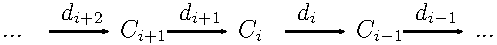
\includegraphics{chain.pdf}
\end{center}

The condition $d_{i-1}d_i=0$ is equivelant to
%requiring $\text{image}(d_i) \subseteq \text{kernel}(d_{i-1})$.
requiring the image of $d_i$ to be contained within the kernel of $d_{i-1}$:

\begin{center}
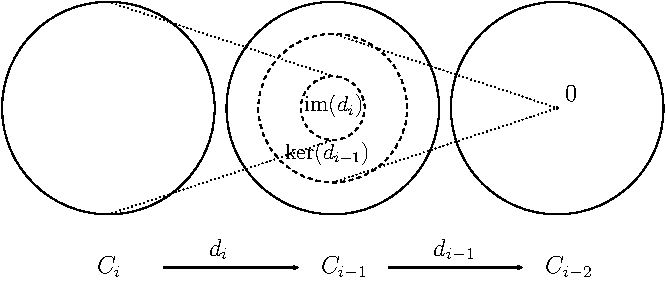
\includegraphics{figure_02.pdf}
\end{center}

Elements of the space $ B_i := \im(d_{i+1}) $ are known as {\it boundaries},
and elements of $ Z_i := \ker(d_i) $ are also known as {\it cycles}.

We form the quotient vector space
$\H_i(C) := B_i(C) / Z_i(C)$,
%$H_i := im(d_{i+1}) / kern(d_i)$,
called the i'th homology 
%vector space.
group (the group operation is given by the vector space addition.)
%We use a different font to dissambiguate the parity
%check matrix, which gets the regular font $H$.

The sequence of spaces ${\H_i}$ will also be denoted as
simply $\H.$ It can be taken to be a chain
complex with the zero boundary map.

We can always consider finite length chain complexes
by appending/prepending zero vector spaces and maps,
for example $A \to B \to C$ can be extended as

    $$ ... \to 0 \to A \to B \to C \to 0 \to ... $$


\subsection{Chain maps}

A chain map $f:C\to C'$ is a sequence of linear maps
$f_i:C_i\to C'_i$ that commute (intertwine) with the boundary map:
$f_{i-1}d_i = d'_if_i.$
Or in diagram form:

\begin{center}
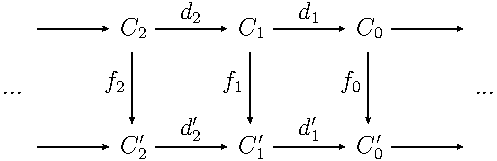
\includegraphics{chainmap.pdf}
\end{center}

The main point about
a chain map is that it
induces a (linear) map of homology groups:

    $$\tilde{f}_i : \H_i\to\H'_i.$$



\subsection{The Hom functor}

%We consider the action of the boundary
%operator by pre-composition:

We consider the boundary operator acting
by pre-composition:

\begin{center}
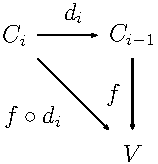
\includegraphics{compose.pdf}
\end{center}

Given a chain complex $C$ and an arbitrary vector
space $V$ we see that the boundary
map $d_i$ acts on maps $f:C_{i-1}\to V$ to give a map $C_i\to V.$
We will fix $V$ to be the underlying field $\Z_2$ then
this action is ``multiplying on the right'',
ie. the transpose operation.
In this way we construct the dual cochain.


\begin{center}
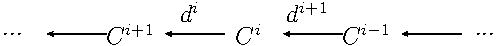
\includegraphics{cochain.pdf}
\end{center}

This is the familiar covector construction.
In general, the so-called hom functor reverses the
direction of all the arrows (of some diagram.)
In our case this means simply that the transpose of a
product reverses the product: $(AB)^\top = B^\top A^\top.$

% ----------------------------------------------------------------
%
%
%
% ----------------------------------------------------------------


% Put this in the intro ??
%
%\subsection{Topologies give chain complexes}
%
%Homology theory in algebraic topology
%
%The boundary of a disc is a circle.
%The boundary of a circle is empty.
%A circle on a sphere is the boundary of a disc,
%but on a torus a circle may not always bound a disc.
%The homology of a space measures the failure of cycles to
%bound a higher dimensional object.
%
%% *** figure here ***
%
%There are many ways to carve up a space such that
%we can perform arithmetic (linear combinations) on
%finite dimensional objects within.
%Definition of n-dimensional object and it's
%(n-1)-dimensional boundary, such that these
%boundaries have trivial boundary themselves.
%
%Cubical (or simplicial) singular homology.
%\cite{Massey}.


\subsection{Classical linear codes}

A classical linear code may be specified as the
kernel of a parity check matrix $\S:\Z_2^n\to \Z_2^m.$
As a chain complex, this is the homology group at
$\Z_2^m.$

As a notational convenience we will sometime denote
a vector space by its (integer) dimension,
eg. $\S:n\to m.$

\setlength{\tabcolsep}{15pt}

\begin{center}
\begin{tabular}{ c c }
\underline{Chain}           &   \underline{Cochain}       \\[8pt]
%$\S:n\to m$      &      $\S^\top:m\to n$    \\[8pt]
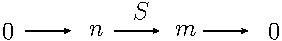
\includegraphics{classchain.pdf}   &  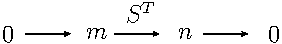
\includegraphics{classcochain.pdf} \\[8pt]
$\H_1=\ker(\S)=:L$  &   $\H^0=\ker(\S^\top) =: L^\top $   \\[8pt]
$\H_0=m/{\im(\S)}=\coker(\S)$ &     $\H^1=n/{\im(\S^\top)}=\coker(\S^\top)$     \\[8pt]
\end{tabular}
\end{center}


\subsection{Quantum stabilizer codes}


A quantum (CSS) code is given by two parity
check matrices $\S_X:n\to m_X$ and $\S_Z:n\to m_Z,$
such that the chain condition $ \S_X \S_Z^\top = 0$
is satisfied.


\begin{center}
\begin{tabular}{ c c }
\underline{Chain}           &   \underline{Cochain}       \\[8pt]
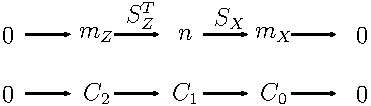
\includegraphics{quchain.pdf}     &  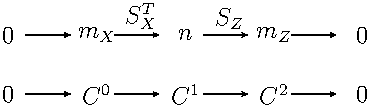
\includegraphics{qucochain.pdf} \\[8pt]
$\H_2=\ker(\S_Z^\top)$                &   $\H^0=\ker(\S_X^\top) $   \\[8pt]
$\H_1=\ker(\S_X)/\im(\S_Z^\top)=:L_X$  &   $\H^1=\ker(\S_Z)/\im(\S_X^\top) =: L_Z $   \\[8pt]
$\H_0=m_X/{\im(\S_X)}=\coker(\S_X)$             &   $\H^2=m_Z/{\im(\S_Z)}=\coker(\S_Z)$     \\[8pt]
\end{tabular}
\end{center}

In the chain we are thinking of the space
$m_Z$ as the space of ``2-dimensional'' objects.
In the toric code this is the space of plaquettes,
but more generally we can think of these as ``generator
labels''. The space $n$ is associated with the physical
qubits, this is where the pauli operators reside.

\begin{center}
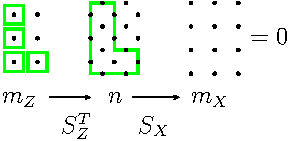
\includegraphics{toric_mZ.pdf}
\end{center}

In the toric code $n$ is the space of ``1-dimensional'' error
operators. The space $m_X$ is then the space of
(X-type) syndrome measurements. In the toric code
these are the ``zero-dimensional'' end-points of (Z-type)
error operators.

\begin{center}
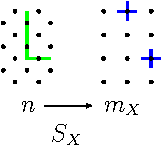
\includegraphics{toric_mX.pdf}
\end{center}


% ----------------------------------------------------------------
%
%
%
% ----------------------------------------------------------------



\section{Tensor product}


The tensor product $C\otimes C'$ of two chain complexes $(C, d)$ and $(C', d')$
is given by

%    $$ (C\otimes C')_i = \bigoplus_{j+k=i} C_j\otimes C'_k $$
    $$ (C\otimes C')_i = \sum_{j+k=i} C_j\otimes C'_k $$

%This is a sum along the diagonals, for example:

with boundary map

    $$ d(c\otimes c') = d(c)\otimes c' + (-1)^{deg(c)}c\otimes d'(c').$$


%We now consider the following two dimensional diagram
%formed from two chain complexes $C$ and $C'$:

%We would like to form a product $C\otimes C'$ of two chain
%complexes $C$ and $C'$. To this end consider the following
%diagram:

To motivate these formulae, consider the following
two dimensional complex:

\begin{center}
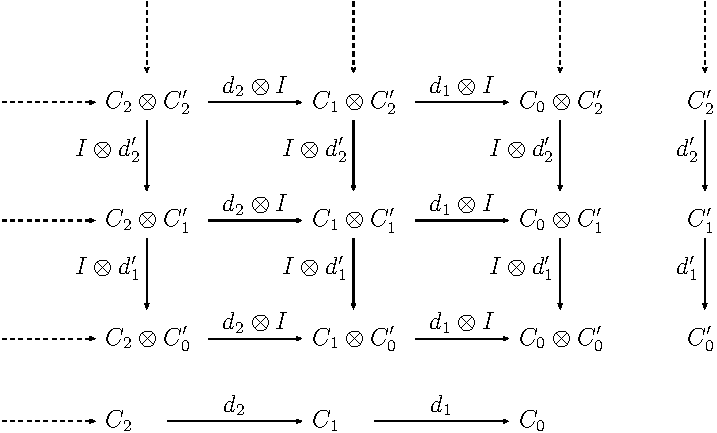
\includegraphics{figure_03.pdf}
\end{center}

where $I$ indicates the appropriate identity map on each vector space.

To reduce this to a one dimensional structure we
(direct) sum along the diagonals, for example:

%Tensor product of two length three chain complexes
\begin{center}
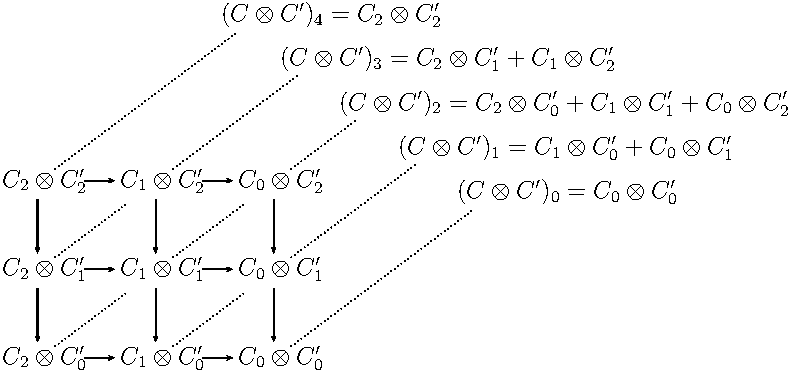
\includegraphics{figure_04.pdf}
\end{center}

Now we add the arrows in an alternating fashion to get a boundary map.
The composition of two arrows in the same direction is
evidently zero, and
we use an alternating weight 
to force the two paths around each square to cancel:

\begin{center}
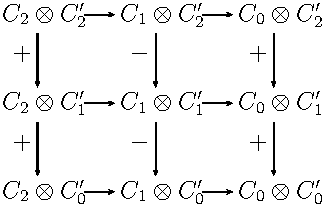
\includegraphics{figure_05.pdf}
\end{center}

With this definition of tensor product the category of
chain complexes becomes a monoidal category 
(See \cite{Baez09}, section 2.3 for a helpful discussion of
monoidal categories.)
%For the categorical definition of the tensor
%product see \cite{Baez09}, section 2.3.

\subsection{The Kunneth formula}

The homology group of the product inherits the same structure
as the underlying chain complex.
This is the import of the Kunneth formula:

    $$ \H_i(C\otimes C') = \sum_{j+k=i} \H_j(C) \otimes \H_k(C') $$

We now define a homomorphism
$ f:\H(C)\otimes \H(C') \to \H(C\otimes C')$
by its action on the subspaces: 
    $$ f:\H_j(C)\otimes \H_k(C') \to \H_{j+k}(C\otimes C').$$

defined by choosing $u_j\in \ker(d_j), u'_k\in \ker(d'_k)$
and then noting that 
    $$ (d_j\otimes I)(u_j\tensor u'_k) = 0,\ \ 
        (I\otimes d'_k)(u_j\tensor u'_k) = 0 $$
which means $u_j\tensor u'_k$ is in the kernel
of the tensor product boundary map, and so represents
an element of $\H_{j+k}(C\otimes C').$
Next check that the choice of $u_i, u'_j$ did not matter...

Weight of stabilizers...
Weight of logops...


\subsection{Product of two classical codes}


The hypergraph product of Tillich and Zemor \cite{Tillich09} is the
product of a classical code and the dual of a classical code.
We didn't define such a product above, but evidently if we
follow the arrows in the same way (or alternativy,
relabel the cochain) it should all work out.

\begin{center}
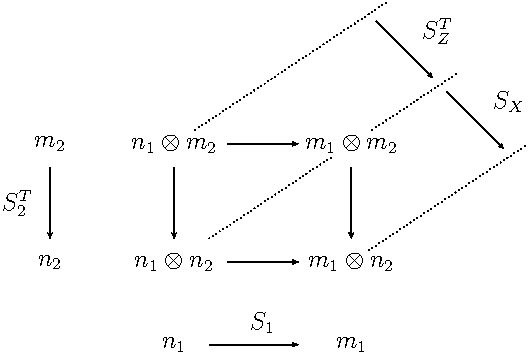
\includegraphics{hyperprod.pdf}
\end{center}

We use the Kunneth formulae to compute the logical
operators:

\begin{align*}
%    \H_1(C_1\otimes C_2^\top)   &= m_1/\im(\S_1)\otimes L_2^\top + L_1 \otimes n_2 / \im(\S_2^\top) \cr
    \H_1(C_1\otimes C_2^\top)   &= \coker(\S_1)\otimes L_2^\top + L_1 \otimes \coker(\S_2^\top) \cr
    |\H_1(C_1\otimes C_2^\top)| &= (m_1-|\im(\S_1)|)|L_2^\top| + |L_1|(n_2 - |\im(\S_2^\top)|) \cr
        &= (m_1-|\im(\S_1^\top)|)|L_2^\top| + |L_1|(n_2 - |\im(\S_2)|) \cr
        &= |\ker(\S_1^\top)||L_2^\top| + |L_1||\ker(\S_2)| \cr
        &= |L_1^\top||L_2^\top| + |L_1||L_2| \cr
\end{align*}

The toric code is obtained from the product of a
(classical) repitition code with its dual.
The important thing to note is that the parity check
matrix (stabilizer generators) is the object of primary
importance, not the space of logical operators.
To get the toric code we must start with a degenerate
parity check matrix  $
\S = \left(
\begin{array}{ccc}
1 & 1 & 0 \\
0 & 1 & 1 \\
1 & 0 & 1 \\
\end{array}
\right).$ 
Then $|L|=|L^\top|=1$ and we get the two logical
qubits in the product.
Using the matrix $
\S = \left(
\begin{array}{ccc}
1 & 1 & 0 \\
0 & 1 & 1 \\
\end{array}
\right).$ gives $|L|=1, |L^\top|=0$ which gives
one logical qubit in the product; this is a surface
code.

\subsection{Product of a classical and a quantum code}

This results in two separate quantum codes, as indicated in
the following diagram:

\begin{center}
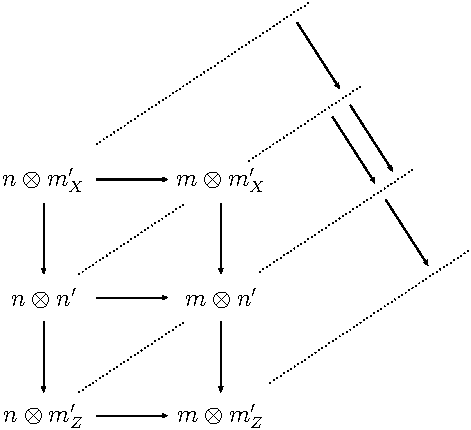
\includegraphics{prodcq.pdf}
\end{center}

(There are also two classical codes at the endpoints.)

In this way we can generate the 3 (spatial) dimension toric code,
as a product of the 2D toric code with the repitition code.
Here we see the two resulting codes have sheets and lines for
logical operators, one code has x-type sheets and z-type lines, the
other code is x-type lines and z-type sheets.

\subsection{Product of two quantum codes}

Continueing this pattern we can generate three different
quantum codes as a product of two quantum codes:

\begin{center}
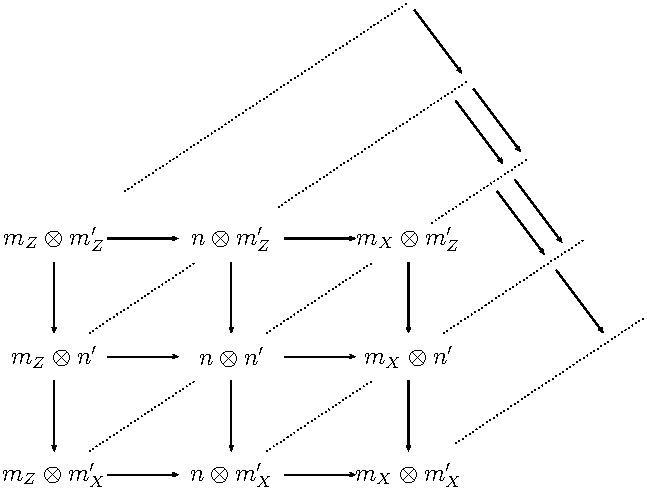
\includegraphics{prodqq.pdf}
\end{center}

For example, the product of the 2D toric code with itself
produces the 4D toric code with x and z type sheet operators,
thats the code in the middle.

Another example, the middle code of the product Stean x Stean has
parameters $[67, 1, 9].$


%\section{Code concatenation}

% ----------------------------------------------------------------
%
%
%
% ----------------------------------------------------------------


\section{Sums and Pushouts}

In any category the sum of two objects $A$ and $B$ is given by
an object $C$ and two maps $f:A\to C$ and $g:B\to C$. These
maps show how to embedd $A$ and $B$ into their ``sum''. A further
requirement is that $C$ is somehow minimal: any other contender
$C'$ for the sum of $A$ and $B$ with ``embedding'' maps $f'$ and $g'$
must factor uniquely through $C$.

In the category of sets we take the disjoint union of $A$ and $B$,
similarly in the category of topological spaces. The embedding
into the sum is the obvious inclusion map.

In the category of vector spaces, we take the direct sum $A\oplus B$, together
with maps $f=I\oplus 0$ and $g=0\oplus I.$
This extends to the category of chain complexes, which 
gives the disjoint union of two codes.

If we would like to join objects $A$ and $B$ along some
``sub-part'', $i:R\to A$, $j:R\to B$ we play the same game
but now require $f$ and $g$ to respect $i$ and $j$, that is,
$f\circ i = g\circ j.$ This is known as a ``pushout'' (of $i$ and $j$.)
In the category of sets, we would take the disjoint union as
before, and then identify those elements according to $(fi)(r) \sim (gj)(r), r\in R.$

This identification also works for topological spaces,
but for vector spaces we project out the {\it subspace} defined
by $fi - gj.$ The notation is then $A\oplus_R B.$

Extended to chain complexes we obtain a general way to
``weld'' two quantum codes together~\cite{Michnicki12}.

TODO...



